\section{Probability}
\subsection{Random Variables}
\begin{itemize}
    \item Values depend on outcomes of a random phenomenon
    \item Random variable $X$ is a variable that takes a numerical value $x$, which depends on a random experiment
    \item \textcolor{blue}{Discrete} $X$ takes any of a finite set of values ${1.5, 2.123, 6.2, 10}$
    \item \textcolor{blue}{Continous} $X$ takes any value of an uncountable range e.g. real numbers from an interval
\end{itemize}
\vspace{10pt}
\textbf{Best we can know}
\begin{itemize}
    \item All possible values
    \item Probability of each value
\end{itemize}
E.g. The discrete random variable $X$ is the number observed when rolling a fair dice.\\
$P(X=x)$ = $P(x)$: $1/6$ for each possible value \\

\textbf{Joint Probability}
\begin{itemize}
    \item Joint Properties of two random variables
    \item Defined by the Joint Probability Mass Function
\end{itemize}
E.g. Dice1 = 5 \textcolor{blue}{and} Dice2 = 4\\
$P_{XY}(5,4) = P_X(5) * P_Y(4) = 1/6 * 1/6 = 1/36$\\
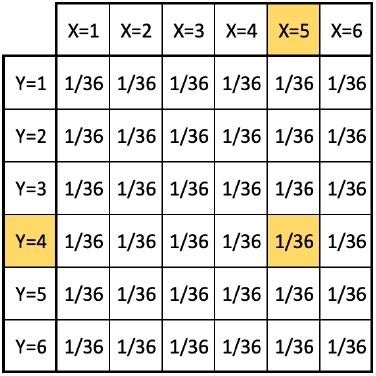
\includegraphics[width=0.5\linewidth]{joint_probability.png} \\

\textcolor{blue}{Independant random Variables}

Joint Probability is the product of the individual probabilities

\begin{center}
    $P(X,Y) = P(X) * P(Y)$

    $P(X,Y,Z) = P(X) * P(Y) * P(Z)$
\end{center}
\vspace{10pt}
\textbf{Marginal Probability} \\
Marginal probability is the probability of an event irrespective of
the outcome of another variable. Can be calculated from the
Joint Probability. (Ganze Spalte/Zeile von Joint Probability addieren = Summe, anderes ignorieren) \\

\textbf{Conditional Probability}
\begin{itemize}
    \item One variable is no longer random
    \item X is observed, its value is fixed
    \item Calculate the probabilities of Y given X: $P(Y | X)$
\end{itemize}
\vspace{10pt}
\textcolor{blue}{Correlated random Variables}
\begin{itemize}
    \item There are events that are not independant
    \item Such random variables are correlated
    \item $X$: observe clouds (0=no, 1=small, 2=big)
    \item $Y$: observe rain (0=no, 1=light, 2=moderate, 3=heavy)
\end{itemize}
\vspace{10pt}
\textcolor{red}{Important: Do not just read the selected data point (e.g. 0.05), if the total value of the column is not 1}

E.g. $P(Y | X) = 0.05 / 0.35 (column sum) = 0.1428 = 14.28\%$ \\

\begin{center}
    $P(X, Y) = P(X | Y) * P(Y)$

    $P(X, Y) = P(Y | X) * P(X)$

    $P(Y | X) = \frac{P(X,Y)}{P(X)}$
\end{center}
\vspace{10pt}
\textbf{Bayes Rule}

$P(X|Y)*P(Y) = P(Y|X)*P(X)$

Therefore

$P(Y|X) = \frac{P(X|Y)*P(Y)}{P(X)}$


\subsection{Probability mass function (PMF)}
Wahrscheinlichkeitsfunktion, a function f(x) that provides the probability for each value x of a discrete random
variable $X$ \\

Graph of a PMF \\
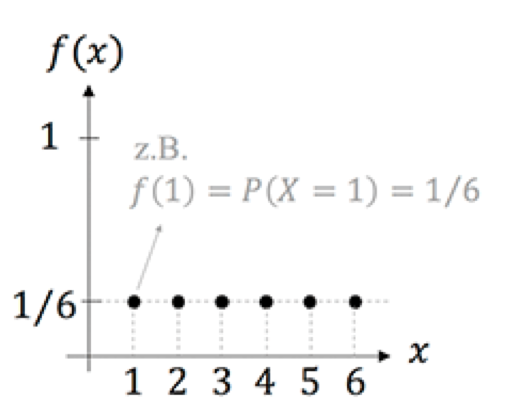
\includegraphics[width=0.4\linewidth]{pmf-graph.png} \\

\textbf{Uniform Distribution}

Wert im Intervall ist gleich wahrscheinlich. Werte ausserhalb Intervall sind \textcolor{blue}{nicht} möglich \\


\textbf{Gaussian Distribution}

Normal-/Glocken-Distribution

$[-1\sigma; 1\sigma] =$ \textcolor{blue}{68.2\%}

$[-2\sigma; 2\sigma] =$ \textcolor{blue}{95\%}

$[-3\sigma; 3\sigma] =$ \textcolor{blue}{99.7\%}
